% Created 2025-04-02 Wed 20:09
% Intended LaTeX compiler: pdflatex
\documentclass[11pt]{article}
\usepackage[utf8]{inputenc}
\usepackage[T1]{fontenc}
\usepackage{graphicx}
\usepackage{longtable}
\usepackage{wrapfig}
\usepackage{rotating}
\usepackage[normalem]{ulem}
\usepackage{amsmath}
\usepackage{amssymb}
\usepackage{capt-of}
\usepackage{hyperref}
\author{aishift}
\date{\today}
\title{Mimi president}
\hypersetup{
 pdfauthor={aishift},
 pdftitle={Mimi president},
 pdfkeywords={},
 pdfsubject={},
 pdfcreator={Emacs 31.0.50 (Org mode 9.7.11)}, 
 pdflang={English}}
\begin{document}

\maketitle
\tableofcontents

\section{Closed beta}
\label{sec:orgae7e1b9}
\subsection{Problem}
\label{sec:orge1438fd}

The rapidly developing Cyber Valley project has diverse sources of truth represented in the following resources:

\begin{itemize}
\item X.com tweets
\item Telegram group chat messages
\item Logseq knowledge base git repositories
\item GitHub issues
\end{itemize}

Searching all of them becomes a time-consuming process and requires a simple way of querying all of them at one time.
\subsection{Solution}
\label{sec:org342b027}

\subsubsection{Announce}
\label{sec:org277f696}

Develop RAG over all resources mentioned in the problem statement and provide an LLM-driven chat bot, which allows interactive and free-form querying of all of them at once.
\subsubsection{Implementation details}
\label{sec:org85e3245}

\begin{enumerate}
\item Embedding model
\label{sec:org92a7a53}

We keep in mind that in the future it could be great to change the chosen model, but it requires complete recalculation for the whole dataset (because of different dimensions and algorithms in general). To handle this, we will store all source data "as is", so making embeddings will be a question of computation.
For the POC we will stick to the OpenAI \href{https://platform.openai.com/docs/guides/embeddings\#embedding-models}{text-embedding-3-small} which is pretty cheap and should work well enough.

\begin{center}
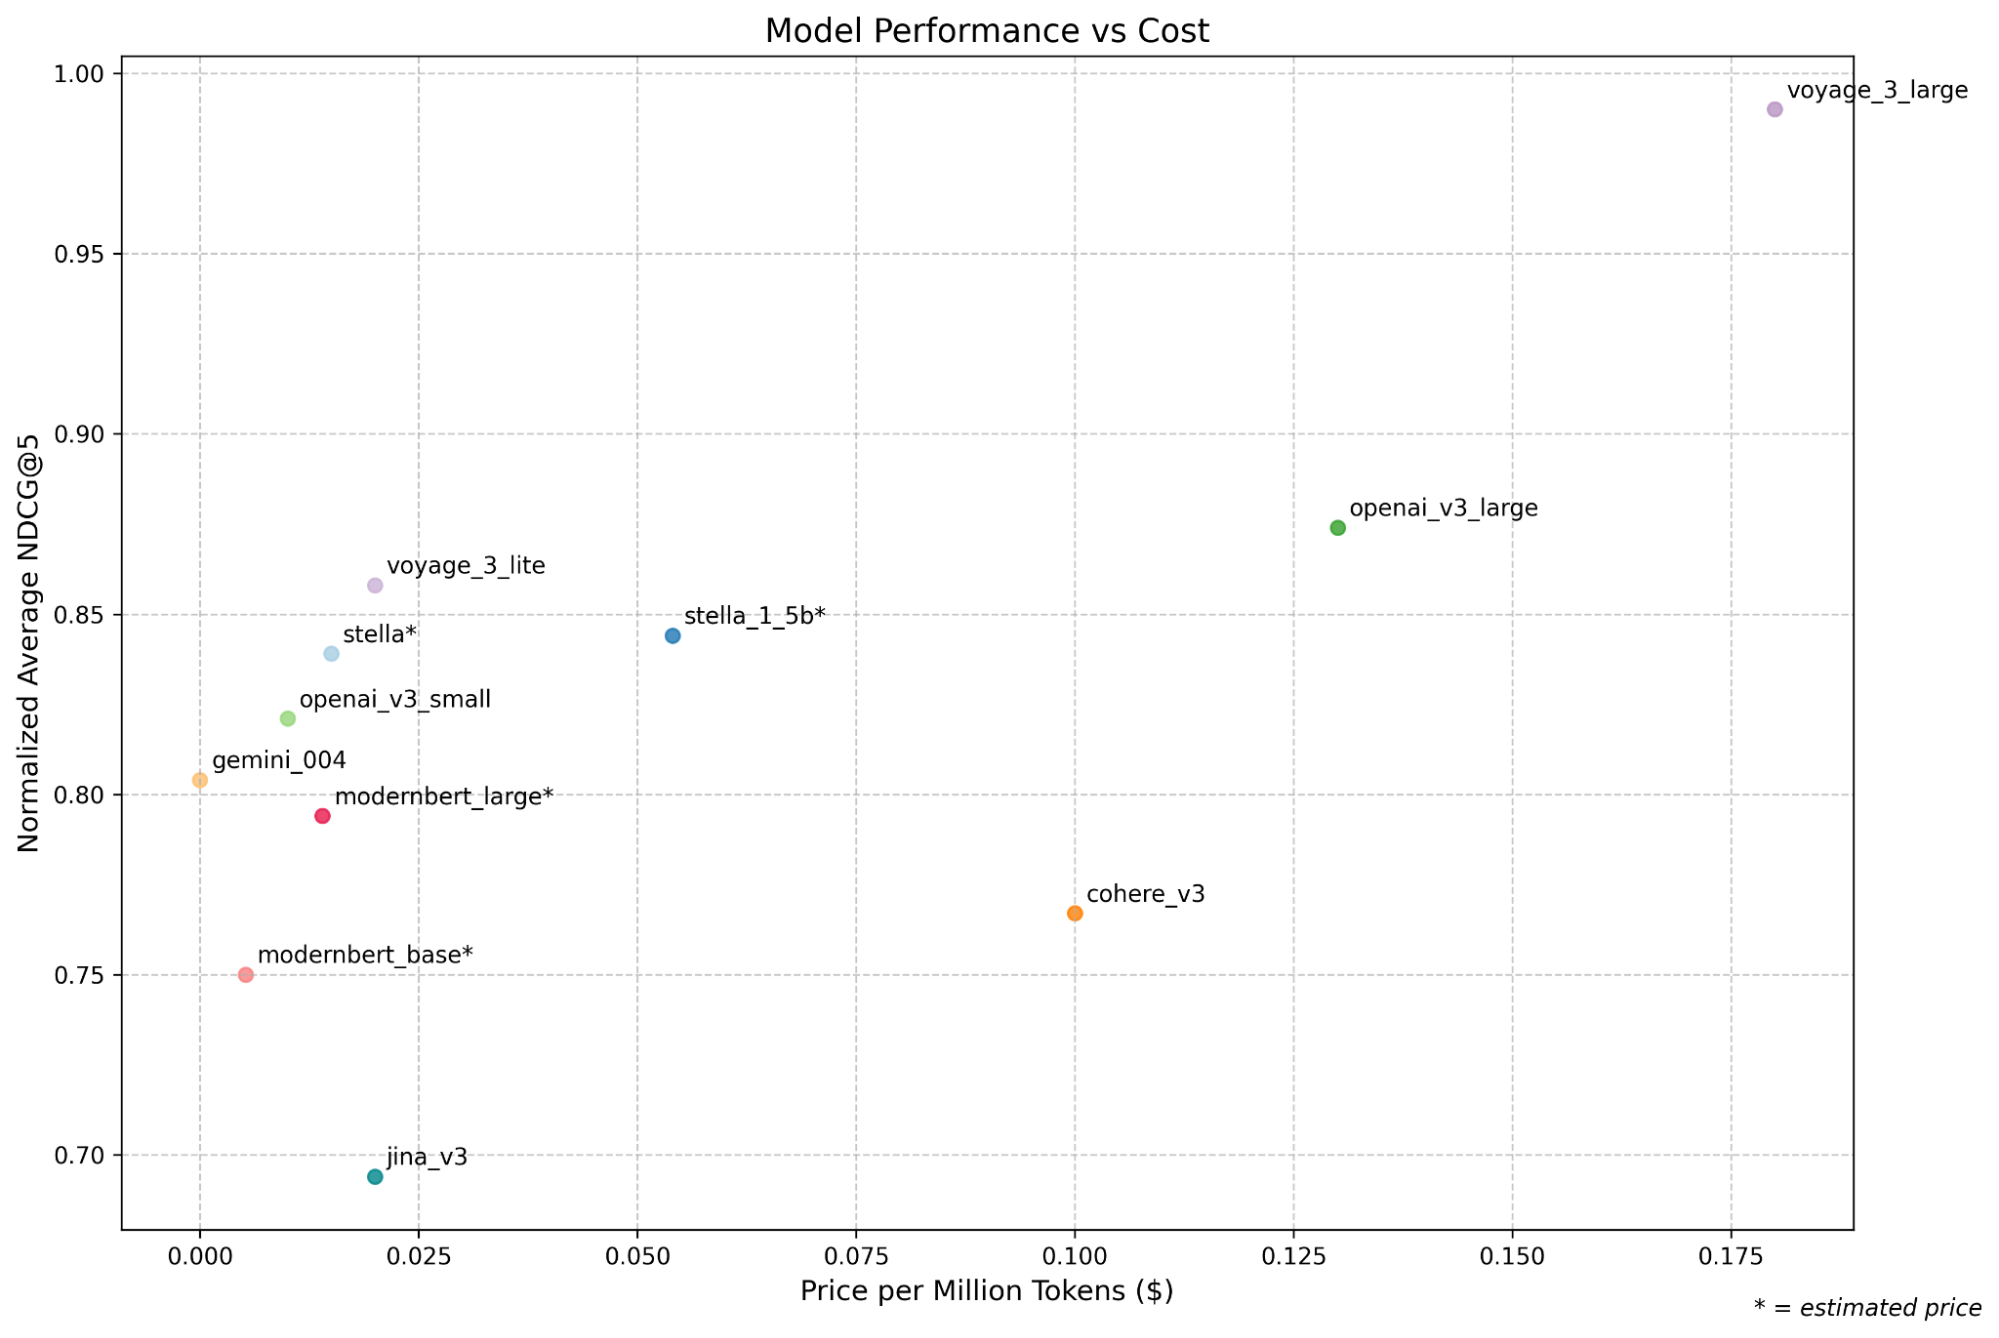
\includegraphics[width=.9\linewidth]{img/embedding-model-pricing.png}
\end{center}
\item LLM chat bot
\label{sec:org7b47951}

Our solution is completely model-agnostic, so any provider could be used and switched on the fly.
\item Data store
\label{sec:org6bc0f34}

We choose \href{https://docs.turso.tech/introduction}{Turso} as our DBMS; it works perfectly with vector search, scales greatly on HDD drives, and has zero network latency because it's built on \href{https://github.com/tursodatabase/libsql/}{libSQL}.
\item Programming language
\label{sec:orgc7cbe91}

We will use Python \& \href{https://www.langchain.com/langchain}{LangChain} for the project because it'll just need glue between IO operations. Rust wouldn't make a visible difference in speed or durability and lacks ready-to-use packages for fast idea testing.
\item Parsing
\label{sec:orge0bb709}

\begin{enumerate}
\item X.com
\label{sec:org470299b}

We don't know for sure the general required number of accounts, their requirements, and their publicity. So for the start and completely for free, it's possible to use Google news RSS. As an example, here is the RSS feed generated for \href{https://x.com/levelsio}{@levelsio} - \url{https://news.google.com/rss/search?q=site:twitter.com/levelsio+when:7}
\item Telegram groups
\label{sec:orgcea1766}

We offer to use the \href{https://core.telegram.org/\#telegram-api}{Telegram Client API}. It requires its own Telegram account but in exchange has access to the whole history of messages (in super groups where it's allowed). The algorithm for adding support for a new group will be the same as adding a new participant to the group. Then we will download all message history (with a given threshold or fully), then listen to new messages and process them as well.
\item GitHub
\label{sec:orge7859f3}

We can use the \href{https://docs.github.com/en/webhooks/webhook-events-and-payloads}{Webhooks API} to get updates on commits to the LogSeq files and issues.
\end{enumerate}
\end{enumerate}
\subsection{Feature improvements}
\label{sec:orgf2afcc7}

\begin{itemize}
\item Embed media (pictures, video, and audio) as well
\item Query and embed provided URLs in the text info
\item Include URLs to the initial sources found with RAG
\item Allow querying only given resources e.g., "What are the statuses of the current projects with aishift in GitHub issues"
\end{itemize}
\section{Minimal valuable product}
\label{sec:org19d7259}

\subsection{Problem}
\label{sec:org74cfde9}

Straight forward RAG solution doesn't work good enough in case of awareness of sources and types of information, so queries about concrete messages in telegram groups or issues assigned to exact people and time boundaries don't work.
\subsection{Solution}
\label{sec:orgca01f65}

Enrich documents metadata with all possible tags and implement additional filtering by them with LLM
\subsubsection{Additional improvements / features}
\label{sec:orga1d7574}

\begin{enumerate}
\item Self aware prompt
\label{sec:org3b8538c}

Make Mimi to know in general in what field of data it operates and what are it's responsibilities
\item Store chat history
\label{sec:org6f67b8c}

Keep each user's conversation so Mimi will know about previous messages
\item Add GitHub project's board parsing
\label{sec:org512339e}

Pure GitHub issues scraping isn't enough, more information should be fetched from the API. TBD @MichaelBorisov
\end{enumerate}
\subsubsection{Implementation details}
\label{sec:org83a6d3b}

\begin{itemize}
\item Migrate from SQLite to \href{https://docs.cozodb.org/en/latest/index.html}{CozoDB} for the better metada search and future easier improves
\item Add context about CyberValley directly to the system prompt
\item Store all chat history in CozoDB as well but take only fixed amount of messages to fit in the context window
\item Improve GitHub scraper to parse more data
\item Use LLM to extract required filters from customer's query and convert them into \href{https://en.wikipedia.org/wiki/Datalog}{Datalog} query
\end{itemize}
\end{document}
